\documentclass[conference]{IEEEtran}
\usepackage{graphicx}
\usepackage{epstopdf}
\usepackage{array}
\usepackage{multirow}
\usepackage{multicol}
\usepackage{empheq}
\usepackage{algorithm}
\usepackage{algorithmicx}
\usepackage{algpseudocode}
\usepackage{amsmath}
\renewcommand{\algorithmicrequire}{ \textbf{Input:}} %Use Input in the format of Algorithm
\renewcommand{\algorithmicensure}{ \textbf{Output:}} %UseOutput in the format of Algorithm
% correct bad hyphenation here
\hyphenation{op-tical net-works semi-conduc-tor}
\begin{document}
\title{Parsing Tables from EDGAR with Python \\and Its Dockerization}
%
% author names and affiliations
\author{\IEEEauthorblockN{Jiali Cheng$^{1}$}
\IEEEauthorblockA{$^{1}$Graduate School of Engineering, Northeastern University, Boston, USA}
}
% make the title area
\maketitle
\begin{abstract}
We use Python to access data from EDGAR, the Electronic Data Gathering, Analysis, and Retrieval system. Given a company ID, called CIK, and an Access Number, called acc-no, an URL to this HTML file is generated. We locate to the 10Q file and extract all the tables and save them as CSV(Comma Separated Values) files. Then we dockerize this pipeline so that it can be used for any websites, not only restricted to IBM.
\end{abstract}
\begin{keywords}
Parse Tabels, HTML, EDGAR, Python, Docker
\end{keywords}
\IEEEpeerreviewmaketitle
%
%Introduction
\section{Introduction}\label{i}
\indent The Electronic Data Gathering Analysis and Retrieval (EDGAR) system is run by Office of Information Technology, U.S. Securities and Exchange Commission. performs automated collection, validation, indexing, acceptance, and forwarding of submissions by companies and others who are required by law to file forms with the SEC. The database is freely available to the public via the Internet (Web or FTP).
\\
\indent In this paper we focus on parsing the tables in the 10Q file of each company. And we introduces a way that given a CIK (company ID), automatically generates the URL (Uniformly Resource Location) to the 10Q file and parse all the tables to save to a CSV file. We then build this pipeline into a Docker image so that it can run on other PCs or laptops. 
\\
\indent Parsing tables have always been a hot topic and a useful tool for data collection. We use 
\\
\indent The remainder of the paper is organized as follows. In Sect.~\ref{ii} we briefly go through the objectives and expectations of the TableParser package and provide an overview of it. Then we detail the design of this package in Sect.~\ref{iii}. Sect.~\ref{iv} presents the results and analysis of the algorithm and code. And in Sect.~\ref{vii} we conclude the report.
\\
%TableParser
\section{System Model}\label{ii}
\indent According to the issues addressed in Sect.~\ref{ii}, we develop a package called TableParser. It basically follows the processing order shown in Fig. ~\ref{flowchart}. Given an Accession Number, we can easily generate the URL of its files on the EDGAR system. And we use regular expression to locate to the 10Q file of this company, which is the target of our parsing job. Then we call the read\_html function to parse the tables out. We clean the noisy data and write it to a CSV file.
\\
%
\begin{figure}
\centering
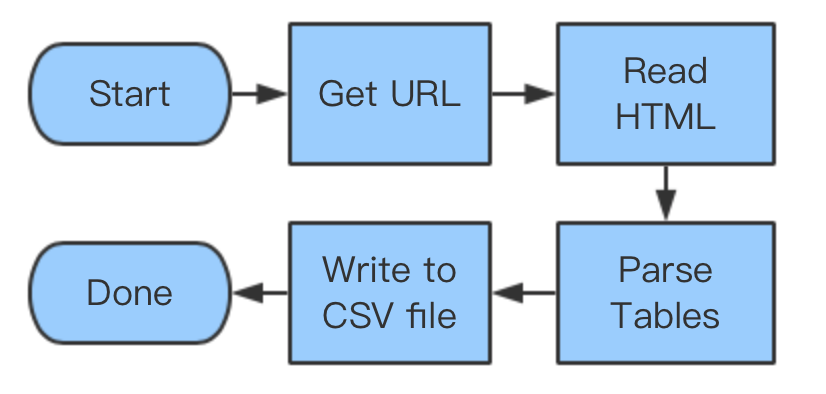
\includegraphics[width=3.8in]{flow1.png}
\caption{The processing flowchart}\label{flowchart}
\end{figure}
%
%Algorithm
\section{The Package}\label{iii}
\indent In this section we describe the detailed design of each part of the package. The package has 2 modules, preparation and parsing. The preparation module basically gets the Accession Number, generates the URL and locates to the 10Q file. And then the parsing module is in charge of extracting the tables and save the items into a CSV file.
\\
\indent First we generate URL according to the given acc\_no. The logic is shown below:
\begin{algorithm}\label{extract}
\caption{Get URL}
\begin{algorithmic}[1]
	\Require acc\_no
	\Ensure 			
	\Function {Get URL} {string acc\_no}
		\State $\Call {getCIK}{acc\_no}$
		\State $\Call {cleanDash}{acc\_no}$
		\State $\Call {generateURL}{acc\_no}$
		\State $\Call {locate\_to\_10q}{url}$ \Comment {Using regular expresion}
	\EndFunction
\end{algorithmic}
\end{algorithm}
\\
\indent Then we delve into the parsing module. As shown in Algorithm ~\ref{extract}, the function $extract()$ takes in the URL of the 10Q file generated by its former part and get the HTTP response. Then it transforms the response into lxml string form for later use. Then we use the package BeautifulSoup to parse all the tables. We utilize the function find\_all that can find all the tags in an HTML string. It is not difficult to draw the basic idea as follow:
\\
\indent 1) Find all the table tags \\
\indent 2) Within each table, find all the 'th' tags, which stands for rows \\
\indent 3) Within each row, find all the 'td' tags, which stands for columns \\
\indent 4) Write each column item into the CSV file \\
which is shown in Algorithm ~\ref{extract}. \\
\indent When an Accession Number is given, the program initiates a unique instance that is related to the Accession Number. If you want to start the parsing process, hit Y and the program will call the the function $start()$, which consists of prepare for the URL of the 10Q file and start extracting. The pseudocode is shown in Algorithm ~\ref{start}.
%
\begin{algorithm}\label{start}
\caption{Start, start running the whole process}
\begin{algorithmic}[1]
	\Ensure double k
	\Function {Master} {double curTime}
		\State $url \gets \Call {FormUrl}{acc-no}$
		\State $url\_10q \gets \Call {FormUrl}{acc-no}$
		\State $\Call {extract}{}$
	\EndFunction
\end{algorithmic}
\end{algorithm}
\indent The result of the parsed tables from the given URL is as follow:
\begin{figure*}
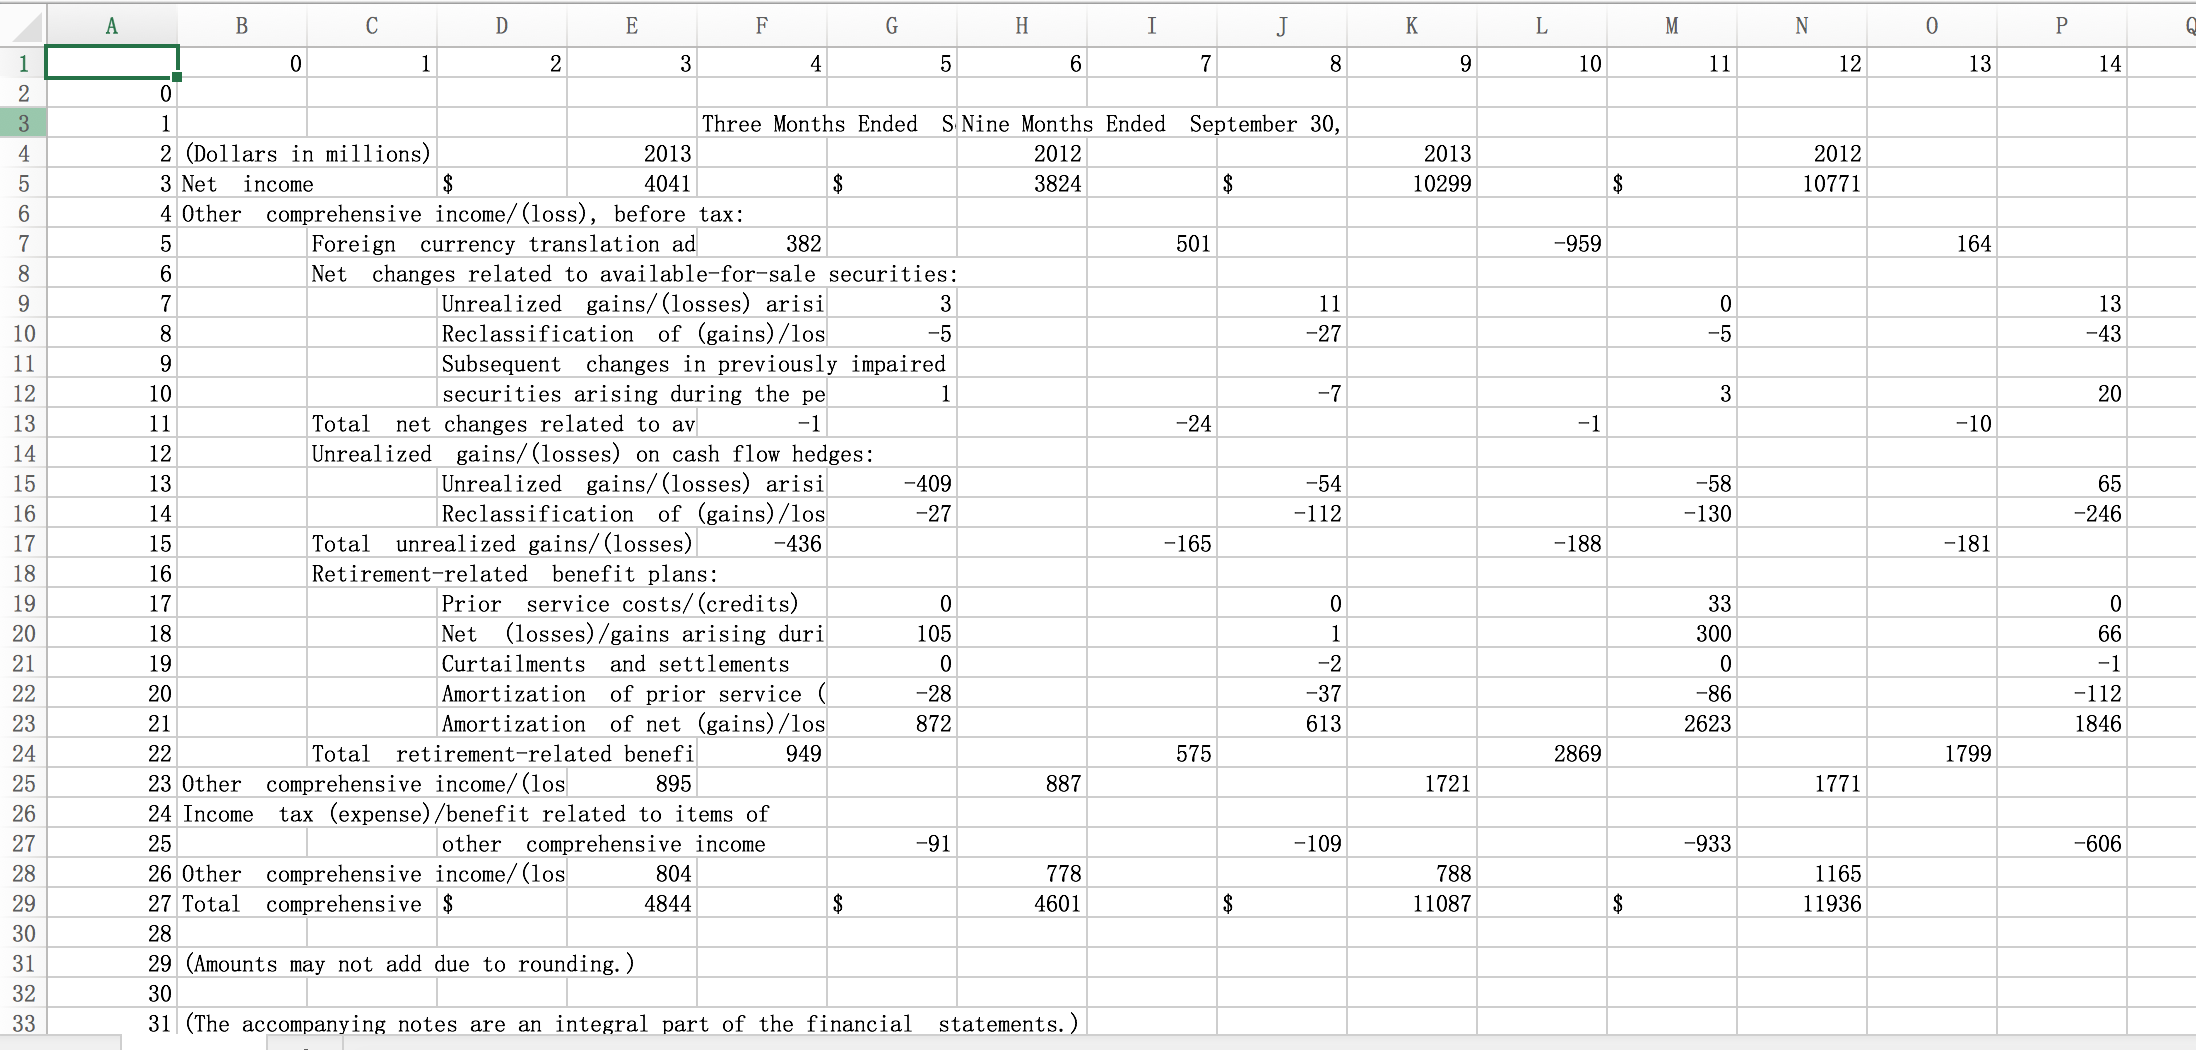
\includegraphics[width=6.0in]{table.png}
\caption{The flow diagram of the LCPR algorithm}\label{data}
\end{figure*}
%
\begin{algorithm}\label{extract}
\caption{Extract, extracting tables from the 10Q file}
\begin{algorithmic}[1]
	\Require url\_10q
	\Ensure double k			\Comment {Get an HTTP response according to the URL of 10Q file and transform the response into lxml form. Then find the HTML tags to get the table items.}
	\Function {Master} {double curTime}
		\State $response \gets \Call {Response}{url\_10q}$
		\State $soup \gets \Call {BeautifulSoup}{response}$
		\State $filename \gets acc-no$
		\State $\Call {Open\_CSV\_File}$
			\For $\Call {Find\_all}{'table'}$
				\For $\Call {Find\_all}{'th'}$
					\For $\Call {Find\_all}{'td'}$
						\State $\Call {Write\_Result}{filename}$
					\EndFor
				\EndFor
			\EndFor
	\EndFunction
\end{algorithmic}
\end{algorithm}
%
\section{Result}\label
\\
%
\section{Conclusion}\label{v}
\indent In this paper, we propose a way to parse tables in the 10Q file of a company in the EDGAR system. Then we dockerize this program to use it on other platforms. Results show that we have finish the job and reach the objectives.%
\begin{thebibliography}{1}
\bibitem{NASA's Space}
Liebrecht, P., Schier, J., Bhasin, K., Bibyk, I., Butler, M., Hudiburg, J., Tai, W., Shames, P., NASA's Space Communications Integrated Architecture, Proceedings of SpaceOps 2010 Conference, AIAA, 25-30 April 2010, Huntsville,
Alabama.
\end{thebibliography}
\end{document} 